\section{System Model and Problem Formulation}
\label{sec:system-model}

\begin{figure}[t]
    \centering
    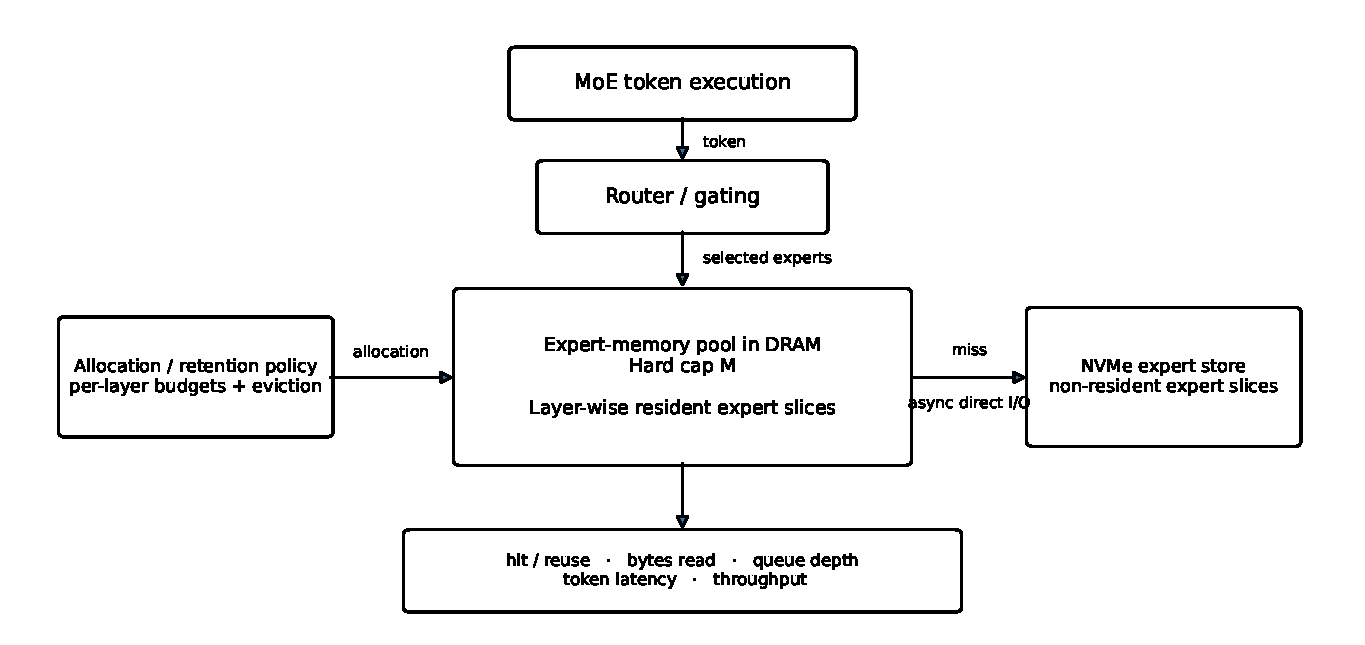
\includegraphics[width=0.96\linewidth]{../docs/figures/argine_system_architecture.pdf}
    \caption{Expert streaming under a hard DRAM budget. For each token, the router selects experts whose weights must reside in a bounded DRAM expert-memory pool. The allocation/retention policy determines per-layer memory budgets and eviction decisions. Requests for non-resident experts trigger asynchronous direct reads from the NVMe expert store. The experiments characterize this coupled allocation-and-retention process through reuse, I/O volume, queue depth, token latency, and generation throughput.}
    \label{fig:architecture}
\end{figure}

\subsection{Expert streaming under a hard memory budget}

We consider autoregressive inference for a sparse mixture-of-experts model with $L$ MoE layers. At layer $l$, a router selects a subset of experts for the current token. Expert weights are stored on NVMe and may be resident in a bounded DRAM pool. Non-expert weights remain resident and are outside the expert-memory budget considered here. Figure~\ref{fig:architecture} summarizes the resulting data path.

\begin{definition}[Expert-memory budget]
The expert-memory budget $M$ is the maximum DRAM capacity available to resident expert weights. It is a hard ceiling enforced by the expert store and is distinct from the memory occupied by non-expert model state, the KV cache, runtime buffers, and the operating system.
\end{definition}

The runtime partitions the expert store into shards, and residency is ultimately enforced at slice granularity. A requested expert is usable only when the required slices can be made resident and pinned for the corresponding computation. A miss therefore triggers storage activity before the dependent computation can proceed. This makes the observed token time a function not only of how much expert memory is resident, but also of which experts are retained and how concurrent I/O requests overlap.

\subsection{Allocation and retention}

Let $M_l$ denote the expert-memory budget assigned to layer $l$. A feasible layer allocation satisfies
\begin{equation}
    M_l \geq 0,
    \qquad
    \sum_{l=1}^{L} M_l \leq M .
    \label{eq:allocation-budget}
\end{equation}
The \emph{allocation} problem chooses the vector
\begin{equation}
    \mathbf{M}=(M_1,\ldots,M_L),
    \label{eq:allocation-vector}
\end{equation}
whereas the \emph{retention} problem chooses which expert slices occupy the capacity assigned to each layer. These are coupled but distinct decisions. Reallocating memory can reduce misses caused by an unfavorable partition even if the replacement rule within a layer is unchanged; conversely, an improved partition cannot remove misses caused by poor retention within the allocated capacity.

This separation motivates the principal policy comparison used later in the paper. Global LRU supplies a conventional recency baseline. Per-layer uniform LRU isolates the effect of partitioning memory equally across layers. The tested \texttt{adaptive-e64} policy changes layer allocations in replay. A Belady-style future-informed reference supplies a deliberately unattainable comparison that quantifies residual selection headroom rather than an implementable online policy.

\subsection{Expert working sets}

For a layer $l$ and a routing trace $W$, let $p_{l,e}(W)$ be the observed fraction of routed selections assigned to expert $e$. Sort experts in decreasing order of $p_{l,e}$. For a coverage target $q\in(0,1)$, define the effective expert working set
\begin{equation}
    \mathrm{EWS}_{q}(l,W)
    =
    \min\left\{
        k:
        \sum_{e=1}^{k} p_{l,(e)}(W) \geq q
    \right\},
    \label{eq:ews}
\end{equation}
where $p_{l,(e)}$ denotes the $e$th largest routing frequency. We report both the expert count and its normalized form
\begin{equation}
    f_{q,l}(W)
    =
    \frac{\mathrm{EWS}_{q}(l,W)}{N_l},
    \label{eq:ews-fraction}
\end{equation}
with $N_l$ the number of routed experts in layer $l$. Section~\ref{sec:heterogeneity} uses $q=0.90$ to characterize layer heterogeneity.

EWS is a demand descriptor, not a cache model. It summarizes concentration over an observed trace but does not encode temporal order, co-activation, expert size, sharding, or I/O overlap. We therefore treat it as one explanatory variable rather than as a sufficient predictor of performance.

\subsection{Normalized pressure and one-token footprint}

To compare memory pressure across the two evaluated models, we define a model-specific one-token expert footprint $F$. For each MoE layer, the router selects $k_l$ routed experts. Let $s_{l,e}$ be the expert-store bytes required for one expert of that layer, including the gate, up, and down slices after the store's alignment rule. Then
\begin{equation}
    F
    =
    \sum_{l=1}^{L} k_l s_l ,
    \label{eq:footprint}
\end{equation}
where $s_l$ is the per-expert stored size for layer $l$. The 80B model's shared expert is not part of the expert store and is therefore excluded from $F$.

For the evaluated quantized models, the derived footprints are
\begin{equation}
    F_{30}=1{,}097{,}072{,}640~\mathrm{B}
    \approx 1.0217~\mathrm{GiB},
    \qquad
    F_{80}=719{,}585{,}280~\mathrm{B}
    \approx 0.6702~\mathrm{GiB}.
    \label{eq:footprints}
\end{equation}
We use
\begin{equation}
    \rho = \frac{M}{F}
    \label{eq:normalized-pressure}
\end{equation}
as a physically motivated pressure coordinate in the extreme-pressure and matched-pressure experiments. Importantly, $F$ is a derived scale, not a claimed feasibility threshold. Section~\ref{sec:pressure-regimes} directly tests that distinction.

\subsection{Metrics and performance quantities}

We distinguish three classes of measurements.

\paragraph{Reuse.}
Expert-level reuse describes whether the expert demand represented by a routing event is already resident under the relevant replay or diagnostic semantics. Runtime-style hit accounting instead follows the expert store's slice-level bookkeeping. The two quantities are related but not interchangeable.

\paragraph{I/O.}
We record bytes read, read count, and queue-depth information. Queue depth matters because misses can overlap: the wall-clock cost of an additional miss depends on how much of its I/O is hidden behind other reads or computation.

\paragraph{End-to-end performance.}
The principal runtime quantities are generation throughput in tokens/s and its reciprocal token latency in ms/token. Time-to-first-token and prompt throughput are reported where relevant but are not the primary optimization target in the results presented here.

The central systems question can therefore be stated more precisely than ``how much of the model fits in memory'': given a hard expert-memory budget $M$, how should memory be allocated across layers and retained within those allocations so as to minimize the \emph{time cost} of non-resident expert demand?
